\documentclass[14pt, compress, aspectratio=1610, c, professionalfonts]{beamer}

\title{Macroevolution of ecological networks}
\author{Timoth\'ee Poisot}
\date{\today}
\institute{UC}

\usecolortheme{plab}
\usetheme{plab}

% Convex path
\newcommand{\convexpath}[2]{
  [   
  create hullcoords/.code={
    \global\edef\namelist{#1}
    \foreach [count=\counter] \nodename in \namelist {
      \global\edef\numberofnodes{\counter}
      \coordinate (hullcoord\counter) at (\nodename);
    }
    \coordinate (hullcoord0) at (hullcoord\numberofnodes);
    \pgfmathtruncatemacro\lastnumber{\numberofnodes+1}
    \coordinate (hullcoord\lastnumber) at (hullcoord1);
  },
  create hullcoords
  ]
  ($(hullcoord1)!#2!-90:(hullcoord0)$)
  \foreach [
  evaluate=\currentnode as \previousnode using \currentnode-1,
  evaluate=\currentnode as \nextnode using \currentnode+1
  ] \currentnode in {1,...,\numberofnodes} {
    let \p1 = ($(hullcoord\currentnode) - (hullcoord\previousnode)$),
    \n1 = {atan2(\y1,\x1) + 90},
    \p2 = ($(hullcoord\nextnode) - (hullcoord\currentnode)$),
    \n2 = {atan2(\y2,\x2) + 90},
    \n{delta} = {Mod(\n2-\n1,360) - 360}
    in 
    {arc [start angle=\n1, delta angle=\n{delta}, radius=#2]}
    -- ($(hullcoord\nextnode)!#2!-90:(hullcoord\currentnode)$) 
  }
}

\begin{document}
\tikzstyle{every picture}+=[remember picture]
\everymath{\displaystyle}

\maketitle

\begin{frame} % WTF are networks
   \centering
   \begin{tikzpicture}[auto,
         sp/.style={draw, very thick, minimum size=1.3cm, color=plFg, circle, inner sep=1pt, outer sep=0pt, fill=plBg},
         ssp/.style={draw, very thick, minimum size=1.0cm, color=plYellow, circle, inner sep=1pt, outer sep=0pt, fill=plBg},
         int/.style={draw, shorten >= 2pt, shorten <= 2pt, ->, >=latex', thick},
         sint/.style={draw, shorten >= 2pt, shorten <= 2pt, ->, >=latex', thick}
      ]
      \node[sp] at (0,0) (trex) {\includegraphics[width=1.2cm]{images/trex.png}};
      \node[sp, below=0.8cm of trex] (wolf) {\includegraphics[width=0.8cm]{images/wolf.png}};
      \node[sp, below=0.8cm of wolf] (deer) {\includegraphics[width=0.8cm]{images/deer.png}};
      \node[sp, below right=0.8cm and 0.8cm of deer] (fern) {\includegraphics[width=0.8cm]{images/fern.png}};
      \node[sp, above right=0.8cm and 0.8cm of fern] (apis) {\includegraphics[width=0.8cm]{images/apis.png}};
      \node[sp, above=0.8cm of apis] (wasp) {\includegraphics[width=0.8cm]{images/wasp.png}};

      \draw[int] (trex) -- (wolf);
      \draw[int] (wolf) -- (deer);
      \draw[int, color=plGreen] (deer) -- (fern);
      \draw[int, <->, color=plMagenta] (fern) -- (apis);
      \draw[int, color=plBlue] (wasp) -- (apis);

      \uncover<2->{
      \node[ssp, color=plCyan, fill=plBg, below right=1pt and 3.3cm of apis] (a1) {\includegraphics[width=0.6cm]{images/apis.png}};
      \node[ssp, color=plCyan, fill=plBg, right=0.8cm of a1] (a2) {\includegraphics[width=0.6cm]{images/apis.png}};
      \node[ssp, color=plCyan, fill=plBg, right=0.8cm of a2] (a3) {\includegraphics[width=0.6cm]{images/apis.png}};
      \node[ssp, color=plCyan, fill=plBg, right=0.8cm of a3] (a4) {\includegraphics[width=0.6cm]{images/apis.png}};
      
      \node[ssp, above right=1pt and 3.3cm of wasp] (w1) {\includegraphics[width=0.6cm]{images/wasp.png}};
      \node[ssp, right=0.8cm of w1] (w2) {\includegraphics[width=0.6cm]{images/wasp.png}};
      \node[ssp, right=0.8cm of w2] (w3) {\includegraphics[width=0.6cm]{images/wasp.png}};
      \node[ssp, right=0.8cm of w3] (w4) {\includegraphics[width=0.6cm]{images/wasp.png}};

      \draw[sint] (w1) -- (a1);
      \draw[sint] (w1) -- (a2);
      \draw[sint] (w1) -- (a4);
      \draw[sint] (w2) -- (a2);
      \draw[sint] (w2) -- (a3);
      \draw[sint] (w3) -- (a4);
      \draw[sint] (w4) -- (a4);
   
      \begin{pgfonlayer}{background}
         \uncover<2>{\draw[fill=plFg!30!plBg,draw=none] \convexpath{wasp, w1, w4, a4, a1, apis}{0.8cm};}
      \end{pgfonlayer}

      }


   \end{tikzpicture}
\end{frame}

\begin{frame} % Question
   \centering
   \begin{tikzpicture}[node distance=1.5cm, auto,
      tp/.style={draw, circle, thick, minimum size=0.8cm, color=plGreen},
      bt/.style={draw, circle, thick, minimum size=0.8cm, color=plMagenta},
      flow/.style={->, very thick, >=latex'},
      ]
      % First network
      \node[tp] (t1) {};
      \node[bt, below=1.0cm of t1] (l1) {};
      \draw[flow] (t1) -- (l1);
      % Second network
      \node[tp, right=5.0cm of t1] (t2) {};
      \node[tp, right of=t2] (t3) {};
      \node[tp, right of=t3] (t4) {};
      \node[tp, right of=t4] (t5) {};
      \node[bt, right=5.0cm of l1] (l2) {};
      \node[bt, right of=l2] (l3) {};
      \node[bt, right of=l3] (l4) {};
      \node[bt, right of=l4] (l5) {};
      \draw[flow] (t2) -- (l2);
      \draw[flow] (t3) -- (l2);
      \draw[flow] (t3) -- (l3);
      \draw[flow] (t3) -- (l4);
      \draw[flow] (t3) -- (l5);
      \draw[flow] (t4) -- (l5);
      \draw[flow] (t5) -- (l2);
      \draw[flow] (t5) -- (l3);
      \draw[flow] (t5) -- (l4);
      \draw[flow] (t5) -- (l5);
   \end{tikzpicture}
\end{frame}

\begin{frame} % Canonical AD equation
   \centering
   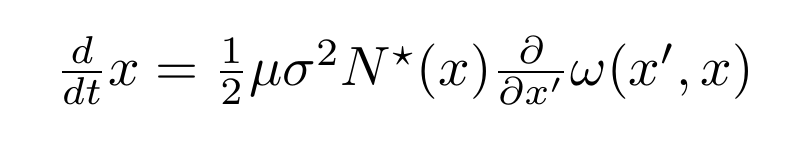
\begin{tikzpicture}
      \node (eq) at (0,0) {\scalebox{2}{
         $\frac{\text{d}}{\text{dt}}x = \frac{1}{2}\mu \sigma^2N^\star(x)\frac{\partial}{\partial x'}\omega(x', x)$
      }};
   \end{tikzpicture}
\end{frame}

\begin{frame} % Explanation of the model
   \centering
   \begin{tikzpicture}[node distance=1.5cm, auto,
      tp/.style={draw, circle, thick, minimum size=0.8cm, color=plGreen},
      bt/.style={draw, circle, thick, minimum size=0.8cm, color=plMagenta},
      net/.style={circle, minimum size=0.5cm},
      flow/.style={->, very thick, >=latex'},
      meta/.style={->, thick, >=latex', plFg!50},
      ]
      % First network
      \node[tp] (t1) {};
      \node[bt, below=1.0cm of t1] (l1) {};
      \draw[flow] (t1) -- (l1);
      % Second network
      \uncover<2->{
      \node[bt, above right=2.0cm and 5.0cm of l1] (l2) {};
      \node[tp, above left=1.0cm and 0.4cm of l2] (t2) {};
      \node[tp, above right=1.0cm and 0.4cm of l2, dashed] (t3) {};
      \draw[flow] (t2) -- (l2);
      \draw[flow, dashed] (t3) -- (l2);
      }
      % Second network with two species
      \uncover<4->{
      \node[bt, right=5.0cm of l2] (l3) {};
      \node[tp, above left=1.0cm and 0.4cm of l3] (t4) {};
      \node[tp, above right=1.0cm and 0.4cm of l3] (t5) {};
      \draw[flow] (t4) -- (l3);
      \draw[flow] (t5) -- (l3);
      }
      % Third network
      \uncover<5->{
      \node[tp, below right=2.0cm and 5.0cm of t1] (t6) {};
      \node[bt, below left=1.0cm and 0.4cm of t6] (l4) {};
      \node[bt, below right=1.0cm and 0.4cm of t6, dashed] (l5) {};
      \draw[flow] (t6) -- (l4);
      \draw[flow, dashed] (t6) -- (l5);
      % Third network with two species
      \node[tp, right=5.0cm of t6] (t7) {};
      \node[bt, below left=1.0cm and 0.4cm of t7] (l6) {};
      \node[bt, below right=1.0cm and 0.4cm of t7] (l7) {};
      \draw[flow] (t7) -- (l6);
      \draw[flow] (t7) -- (l7);
      }

      %% Transitions
      \node[net, below=0.25cm of t1] (n1) {};
      \node[net, above=0.25cm of l2] (n2) {};
      \node[net, above=0.25cm of l3] (n2b) {};
      \node[net, below=0.25cm of t6] (n3) {};
      \node[net, below=0.25cm of t7] (n3b) {};
      \uncover<3->{
      \draw[meta] (n2) edge[bend left=20, shorten >= 1cm, shorten <= 1cm] node [above]{$\epsilon$} (n1);
      }
      \uncover<2->{
      \draw[meta] (n1) edge[bend left=20, shorten >= 1cm, shorten <= 1cm] node {$1-p$} (n2);
      }
      \uncover<4->{
      \draw[meta] (n2) edge[shorten >= 1cm, shorten <= 1cm] node {$1-\epsilon$} (n2b);
      }
      \uncover<5->{
      \draw[meta] (n1) edge[bend left=20, shorten >= 1cm, shorten <= 1cm] node [below]{$p$} (n3);
      \draw[meta] (n3) edge[bend left=20, shorten >= 1cm, shorten <= 1cm] node {$\epsilon$} (n1);
      \draw[meta] (n3) edge[shorten >= 1cm, shorten <= 1cm] node {$1-\epsilon$} (n3b);
      }
   \end{tikzpicture}
\end{frame}

\begin{frame} % Different network metrics
   \centering
   \begin{tikzpicture}[node distance=1.7cm, auto,
      tp/.style={draw, circle, thick, minimum size=0.8cm, color=plGreen},
      bt/.style={draw, circle, thick, minimum size=0.8cm, color=plMagenta},
      flow/.style={->, very thick, >=latex'},
      ]
      \node[tp] (t1) {};
      \node[tp, right of=t1] (t2) {};
      \node[tp, right of=t2] (t3) {};
      \node[tp, right of=t3] (t4) {};
      \node[tp, right of=t4] (t5) {};
      \node[bt, below=1.6cm of t1] (l1) {};
      \node[bt, right of=l1] (l2) {};
      \node[bt, right of=l2] (l3) {};
      \node[bt, right of=l3] (l4) {};
      \node[bt, right of=l4] (l5) {};
      \only<1>{
         \draw[flow] (t1) -- (l1);
         \draw[flow] (t1) -- (l2);
         \draw[flow] (t1) -- (l3);
         \draw[flow] (t1) -- (l4);
         \draw[flow] (t1) -- (l5);
         \draw[flow] (t2) -- (l1);
         \draw[flow] (t2) -- (l2);
         \draw[flow] (t2) -- (l3);
         \draw[flow] (t2) -- (l4);
         \draw[flow] (t3) -- (l1);
         \draw[flow] (t3) -- (l2);
         \draw[flow] (t3) -- (l3);
         \draw[flow] (t4) -- (l1);
         \draw[flow] (t4) -- (l2);
         \draw[flow] (t5) -- (l1);
      }
      \only<2>{
         \draw[flow] (t1) -- (l1);
         \draw[flow] (t1) -- (l2);
         \draw[flow] (t2) -- (l1);
         \draw[flow] (t2) -- (l2);
         \draw[flow] (t3) -- (l3);
         \draw[flow] (t3) -- (l5);
         \draw[flow] (t4) -- (l3);
         \draw[flow] (t4) -- (l4);
         \draw[flow] (t5) -- (l3);
         \draw[flow] (t5) -- (l4);
         \draw[flow] (t5) -- (l5);
      }
      \only<3,4,5,6>{
         \draw[flow,very thin] (t1) -- (l1);
         \draw[flow,very thin] (t1) -- (l2);
         \draw[flow,very thin] (t2) -- (l1);
         \draw[flow,very thin] (t2) -- (l3);
         \draw[flow,very thin] (t3) -- (l2);
         \draw[flow,very thin] (t2) -- (l2);
         \draw[flow,very thin] (t3) -- (l3);
         \draw[flow,very thin] (t3) -- (l5);
         \draw[flow,very thin] (t4) -- (l3);
         \draw[flow,very thin] (t4) -- (l4);
         \draw[flow,very thin] (t5) -- (l3);
         \draw[flow,very thin] (t5) -- (l4);
         \draw[flow,very thin] (t5) -- (l5);
         \only<4>{
            \draw[flow] (t1) -- (l1);
            \draw[flow] (t1) -- (l2);
         }
         \only<5>{
            \draw[flow] (t2) -- (l1);
            \draw[flow] (t2) -- (l2);
            \draw[flow] (t2) -- (l3);
         }
         \only<6>{
            \draw[flow] (t5) -- (l5);
            \draw[flow] (t4) -- (l4);
            \draw[flow] (t5) -- (l4);
         }
      }
   \end{tikzpicture}
\end{frame}

\begin{frame} % Model analysis
   \centering
   \begin{tikzpicture}[trim axis left, trim axis right,
      nd/.style={draw, circle, color=plCyan, very thick, minimum size=0.3cm},
      tn/.style={color=plCyan, very thick}
      ]
      \begin{axis}[
            tick align=outside,
            xmode=log,
            ymin = 0, ymax =1,
            xmin=0.00095, xmax=1,
            xlabel = Probability of losing new interactions,
            xlabel style={yshift=-1em},
            ylabel style={xshift=-1em},
            axis y line*=left, axis x line*=bottom,
            x axis line style={draw opacity=0.0},
            y axis line style={draw opacity=0.0},
            %ymajorgrids,
            axis background/.style={shade,top color=plFg!20, bottom color=plBg, fill opacity=0.1},
            width=12cm, height=8cm
         ]
         \only<1>{ % Connectance
            \addplot [plBlue, only marks] table[x=e, y=Co] {./data/ma.dat};
            % Net 1
            \node [nd] at (axis cs:0.004,0.9) (n1) {};
            \node [nd, left=0.3cm of n1] (n2) {};
            \node [nd, left=0.3cm of n2] (n3) {};
            \node [nd, below=0.3cm of n1] (b1) {};
            \node [nd, below=0.3cm of n2] (b2) {};
            \node [nd, below=0.3cm of n3] (b3) {};
            \draw [tn] (n1) -- (b1);
            \draw [tn] (n1) -- (b2);
            \draw [tn] (n1) -- (b3);
            \draw [tn] (n2) -- (b2);
            \draw [tn] (n2) -- (b3);
            \draw [tn] (n3) -- (b3);
            \draw [tn] (n3) -- (b1);
            % Net 2
            \node [nd] at (axis cs:0.7,0.4) (n1) {};
            \node [nd, left=0.3cm of n1] (n2) {};
            \node [nd, left=0.3cm of n2] (n3) {};
            \node [nd, below=0.3cm of n1] (b1) {};
            \node [nd, below=0.3cm of n2] (b2) {};
            \node [nd, below=0.3cm of n3] (b3) {};
            \draw [tn] (n1) -- (b1);
            \draw [tn] (n2) -- (b2);
            \draw [tn] (n3) -- (b3);
         }
         \only<2>{ % Nestedness
            \addplot [plBlue, only marks] table[x=e, y=NODF] {./data/ma.dat};
            % Net 1
            \node [nd] at (axis cs:0.004,0.6) (n1) {};
            \node [nd, left=0.3cm of n1] (n2) {};
            \node [nd, left=0.3cm of n2] (n3) {};
            \node [nd, below=0.3cm of n1] (b1) {};
            \node [nd, below=0.3cm of n2] (b2) {};
            \node [nd, below=0.3cm of n3] (b3) {};
            \draw [tn] (n1) -- (b1);
            \draw [tn] (n1) -- (b2);
            \draw [tn] (n1) -- (b3);
            \draw [tn] (n2) -- (b1);
            \draw [tn] (n2) -- (b2);
            \draw [tn] (n3) -- (b1);
            % Net 2
            \node [nd] at (axis cs:0.7,0.4) (n1) {};
            \node [nd, left=0.3cm of n1] (n2) {};
            \node [nd, left=0.3cm of n2] (n3) {};
            \node [nd, below=0.3cm of n1] (b1) {};
            \node [nd, below=0.3cm of n2] (b2) {};
            \node [nd, below=0.3cm of n3] (b3) {};
            \draw [tn] (n1) -- (b1);
            \draw [tn] (n2) -- (b2);
            \draw [tn] (n3) -- (b3);
         }
         \only<3>{ % Modularity
            \addplot [plBlue, only marks] table[x=e, y=Q] {./data/ma.dat};
            % Net 1
            \node [nd] at (axis cs:0.004,0.55) (n1) {};
            \node [nd, left=0.3cm of n1] (n2) {};
            \node [nd, left=0.3cm of n2] (n3) {};
            \node [nd, below=0.3cm of n1] (b1) {};
            \node [nd, below=0.3cm of n2] (b2) {};
            \node [nd, below=0.3cm of n3] (b3) {};
            \draw [tn] (n1) -- (b2);
            \draw [tn] (n1) -- (b3);
            \draw [tn] (n2) -- (b1);
            \draw [tn] (n2) -- (b2);
            \draw [tn] (n3) -- (b3);
            % Net 2
            \node [nd] at (axis cs:0.7,0.4) (n1) {};
            \node [nd, left=0.3cm of n1] (n2) {};
            \node [nd, left=0.3cm of n2] (n3) {};
            \node [nd, below=0.3cm of n1] (b1) {};
            \node [nd, below=0.3cm of n2] (b2) {};
            \node [nd, below=0.3cm of n3] (b3) {};
            \draw [tn] (n1) -- (b1);
            \draw [tn] (n2) -- (b2);
            \draw [tn] (n3) -- (b3);
         }
      \end{axis}
   \end{tikzpicture}
\end{frame}

\begin{frame} % ABC in less than 5 seconds
  \centering
  \scalebox{2}{
     $f(\theta) = \mathbf{s}_{\text{sim.}} \hskip 1em \approx \hskip 1em \mathbf{s}_{\text{obs.}}$
  }
\end{frame}

\begin{frame} % Example with one network
   \centering
   \begin{tikzpicture}[trim axis left, trim axis right]
      \begin{axis}[
            tick align=outside,
            xmode=log, ymode=log,
            xlabel = Probability of losing new interactions,
            ylabel = Tendency for specialization,
            xlabel style={yshift=-1em},
            ylabel style={yshift=1em},
            ymin=0.1, ymax=10,
            xmin=0.001, xmax=1,
            axis y line*=left, axis x line*=bottom,
            x axis line style={draw opacity=0.0},
            y axis line style={draw opacity=0.0},
            axis background/.style={shade,top color=plFg!20, bottom color=plBg, fill opacity=0.1},
            width=8cm, height=8cm
         ]
         \addplot[only marks, mark size=0.4, plBlue] table [x=e, y=c]{./data/disp1.dat};
      \end{axis}
   \end{tikzpicture}
\end{frame}

\begin{frame} % All networks
   \centering
   \begin{tikzpicture}[trim axis left, trim axis right]
      \begin{axis}[
            tick align=outside,
            xmode=log, ymode=log,
            xlabel = Probability of losing new interactions,
            ylabel = Tendency for specialization,
            xlabel style={yshift=-1em},
            ylabel style={yshift=1em},
            ymin=0.1, ymax=10,
            xmin=0.001, xmax=1,
            axis y line*=left, axis x line*=bottom,
            x axis line style={draw opacity=0.0},
            y axis line style={draw opacity=0.0},
            axis background/.style={shade,top color=plFg!20, bottom color=plBg, fill opacity=0.1},
            width=8cm, height=8cm,
            legend pos=south west,
            legend cell align=left,
            legend style={fill=none, font=\small, draw=none}
         ]
         \addplot[only marks, mark size=0.9, plGreen] table [x index=1, y index=3]{./data/post_herb.dat}; \addlegendentry{herbivory};
         \addplot[only marks, mark size=0.9, plBlue] table [x index=1, y index=3]{./data/post_poll.dat}; \addlegendentry{pollination};
         \addplot[only marks, mark size=0.9, plRed] table [x index=1, y index=3]{./data/post_disp.dat}; \addlegendentry{dispersal};
         \addplot[only marks, mark size=0.9, plMagenta] table [x index=1, y index=3]{./data/post_para.dat}; \addlegendentry{parasitism};
         \addplot[only marks, mark size=0.9, plYellow] table [x index=1, y index=3]{./data/post_phag.dat}; \addlegendentry{phage};
      \end{axis}
   \end{tikzpicture}
\end{frame}

\begin{frame} % All networks (zoom)
   \centering
   \begin{tikzpicture}[trim axis left, trim axis right]
      \begin{axis}[
            tick align=outside,
            xmode=log, ymode=log,
            xlabel = Probability of losing new interactions,
            ylabel = Tendency for specialization,
            xlabel style={yshift=-1em},
            ylabel style={yshift=1em},
            ymin=1.0, ymax=10,
            xmin=0.01, xmax=1,
            axis y line*=left, axis x line*=bottom,
            x axis line style={draw opacity=0.0},
            y axis line style={draw opacity=0.0},
            axis background/.style={shade,top color=plFg!20, bottom color=plBg, fill opacity=0.1},
            width=8cm, height=8cm,
            legend pos=north east,
            legend cell align=left,
            legend style={fill=none, font=\small, draw=none}
         ]
         \addplot[only marks, mark size=0.9, plGreen] table [x index=1, y index=3]{./data/post_herb.dat}; \addlegendentry{herbivory};
         \addplot[only marks, mark size=0.9, plBlue] table [x index=1, y index=3]{./data/post_poll.dat}; \addlegendentry{pollination};
         \addplot[only marks, mark size=0.9, plRed] table [x index=1, y index=3]{./data/post_disp.dat}; \addlegendentry{dispersal};
         \addplot[only marks, mark size=0.9, plMagenta] table [x index=1, y index=3]{./data/post_para.dat}; \addlegendentry{parasitism};
         \addplot[only marks, mark size=0.9, plYellow] table [x index=1, y index=3]{./data/post_phag.dat}; \addlegendentry{phage};
      \end{axis}
   \end{tikzpicture}
\end{frame}

\begin{frame}[t]{title}
   
\end{frame}

\begin{frame}[b] % Credits
   \small
   \textbf{Image credits:} Maija Karala, Olegivvit, Tracy A. Heath, Adrian Reich, George Starr, Gareth Monger\\
   \texttt{http://creativecommons.org/licenses/by/3.0/}\vskip 1em
   \textbf{Made with:} \LaTeX, pgfplots, tikz\vskip 1em
   \textbf{License:} Creative Commons 4.0 "by" to Timoth\'ee Poisot\\
   \texttt{http://creativecommons.org/licenses/by/4.0/}
   \vskip 1em
\end{frame}

\end{document}
